\section{シミュレーション結果}
シミュレータを用いて、10万回ブラックジャックを行った結果を表\ref{bstable}と表\ref{ratebstable}に示す。
\begin{table}[H]
 \caption{デック数と各戦略での勝利、負け、引き分け\label{bstable}}
 \begin{center}
  \begin{tabular}{|c|c|c|c|c|c|c|}
    \hline & \multicolumn{3}{c|}{デック数無限} & \multicolumn{3}{c|}{デック数1} \\
    \cline{2-7} & 勝ち & 負け & 引き分け & 勝ち & 負け & 引き分け \\
    \hline ベーシックストラテジー & 42746 & 48635 & 8619 & 43111 & 48654 & 8235 \\
    \hline ベーシックストラテジー改変1 & 42583 & 48782 & 8635 & 42923 & 48909 & 8168 \\
    \hline ベーシックストラテジー改変2 & 42223 & 49079 & 8698 & 42955 & 48689 & 8356 \\
    \hline 15以上になるまでヒットする戦略 & 42392 & 49458 & 8150 & 42063 & 50027 & 7910 \\
    \hline 16以上になるまでヒットする戦略 & 41410 & 49506 & 9084 & 41580 & 49672 & 8748 \\
    \hline 17以上になるまでヒットする戦略 & 40870 & 49400 & 9730 & 40974 & 49630 & 9396 \\
    \hline 18以上になるまでヒットする戦略 & 39291 & 52587 & 8122 & 42071 & 49872 & 8057 \\
    \hline
  \end{tabular}
 \end{center}
\end{table}
\begin{table}[H]
 \caption{デック数と各戦略での勝利、負け、引き分けの比率\label{ratebstable}}
 \begin{center}
 \scalebox{0.9}{
  \begin{tabular}{|c|c|c|c|c|c|c|}
    \hline & \multicolumn{3}{c|}{デック数無限} & \multicolumn{3}{c|}{デック数1} \\
    \cline{2-7} & 勝ち(\%) & 負け(\%) & 引き分け(\%) & 勝ち(\%) & 負け(\%) & 引き分け(\%) \\
    \hline ベーシックストラテジー & 42.7 & 48.6 & 8.6 & 43.1 & 48.7 & 8.2 \\
    \hline ベーシックストラテジー改変1 & 42.6 & 48.8 & 8.6 & 42.9 & 48.9 & 8.2 \\
    \hline ベーシックストラテジー改変2 & 42.2 & 49.1 & 8.7 & 43.0 & 48.7 & 8.4 \\
    \hline 15以上になるまでヒットする戦略 & 42.4 & 49.5 & 8.2 & 42.1 & 50.0 & 7.9 \\
    \hline 16以上になるまでヒットする戦略 & 41.4 & 49.5 & 9.1 & 41.6 & 49.7 & 8.7 \\
    \hline 17以上になるまでヒットする戦略 & 40.9 & 49.4 & 9.7 & 41.0 & 49.6 & 9.4 \\
    \hline 18以上になるまでヒットする戦略 & 39.3 & 52.6 & 8.1 & 42.1 & 49.9 & 8.1 \\
    \hline
  \end{tabular}
}
 \end{center}
\end{table}
今回はシミュレータで各戦略を10万回実行した。その結果を勝ち、負け、引き分けの3種類に分けて、表\ref{bstable}と表\ref{ratebstable}にまとめた。表\ref{bstable}は度数で表し、表\ref{ratebstable}では比率で表したものになっている。縦軸はデックの数とそれに対応する勝敗とし、横軸は戦略ごとに分けている。例えば、表\ref{ratebstable}ベーシックストラテジーでデック数1の場合を見ると勝ちが43.1\%で負けが48.7\%で引き分けが8.2\%となっている。\\
全体として勝ちの数は4万回前後に収まっており、負けの数は5万回前後に収まっている。基本的に負けの数のほうが多いことが分かる。デック数で比べると、ほとんどの戦略でデック数1の場合のほうが勝ちの数が多いということが発見される。また、デック数に関係なく、勝ちの数はベーシックストラテジーが一番多い事が分かる。
\bunseki{薩田凱斗}

\section{検定}
先ほどのシミュレーションを行った結果から、ベーシックストラテジーが各戦略の中で最も勝率が高いという事を明らかにする。そのために、各戦略の間の勝率にそれぞれ有意な差があるかどうかを確かめたい。また、デック数によって勝率が変化するということも明らかにする。そのためデック数の違いによって各戦略の勝率にそれぞれ有意な差があるかどうかを確かめるために検定を行う。そこで、それらの推測が実際に正しいかどうかを確かめるために、カイ2乗検定を用いて検証を行った。
\bunseki{薩田凱斗}

\subsection{カイ2乗検定による独立性の検定}
勝率に有意な差があるかどうかを確かめるためカイ2乗検定の独立性の検定を使用する。カイ2乗検定ではカイ2乗値を用いて検定を行う。カイ2乗値は式\ref{kai}で算出する。
\begin{equation} カイ2乗値 = \sum{ \frac{(実現度数 - 理論度数)^2}{理論度数}} \label{kai}\end{equation}
実現度数とは実際に出た度数のことで、理論度数は理想としてでる度数のことである。実現度数はシミュレータの結果から参照し、理論度数はシミュレータの結果から算出する。
理論度数は式\ref{theory}で計算される。
\begin{equation} 理論度数 =  行の合計 ×\frac{列の合計}{すべての合計} \label{theory}\end{equation}
\bunseki{柿崎大輝}

\subsubsection{戦略間の勝率}
カイ2乗検定を行うためにシミュレータの結果の表\ref{kaiinf}を変形する。
\begin{table}[H]
 \caption{デック数無限の場合\label{kaiinf}}
 \begin{center}
  \begin{tabular}{|c|c|c|c|}
    \hline  & 勝ち & 勝ち以外(負けと引き分け) & 合計 \\
    \hline ベーシックストラテジー (実現度数)& 42746 & 57254 & 100000 \\
             ベーシックストラテジー (理論度数)& 41645 & 58355 &  \\
    \hline ベーシックストラテジー改変1 (実現度数)& 42583 & 57417 & 100000 \\
             ベーシックストラテジー改変1 (理論度数)& 41645 & 58355 &  \\
    \hline ベーシックストラテジー改変2 (実現度数)& 42223 & 57777 & 100000 \\
              ベーシックストラテジー改変2 (理論度数)& 41645 & 58355 &  \\
    \hline 15以上になるまでヒットする戦略 (実現度数)& 42392 & 57608 & 100000 \\
             15以上になるまでヒットする戦略 (理論度数)& 41645 & 58355 &  \\
    \hline 16以上になるまでヒットする戦略 (実現度数)& 41410 & 58590 & 100000 \\
             16以上になるまでヒットする戦略 (理論度数)& 41645 & 58355 &  \\
    \hline 17以上になるまでヒットする戦略 (実現度数)& 40870 & 59130 & 100000 \\
             17以上になるまでヒットする戦略 (理論度数)& 41645 & 58355 &  \\
    \hline 18以上になるまでヒットする戦略 (実現度数)& 39291 & 60709 & 100000 \\
             18以上になるまでヒットする戦略 (理論度数)& 41645 & 58355 &  \\
    \hline  合計 & 291515 & 408485 & 700000 \\
    \hline
  \end{tabular}
 \end{center}
\end{table}
\begin{table}[H]
 \caption{デック数1の場合\label{kai1}}
 \begin{center}
  \begin{tabular}{|c|c|c|c|}
    \hline  & 勝ち & 勝ち以外(負けと引き分け) & 合計 \\
    \hline ベーシックストラテジー (実現度数)& 43111 & 56889 & 100000 \\
             ベーシックストラテジー (理論度数)& 42240 & 57760 &  \\
    \hline ベーシックストラテジー改変1 (実現度数)& 42923 & 57077 & 100000 \\
             ベーシックストラテジー改変1 (理論度数)& 42240 & 57760 &  \\
    \hline ベーシックストラテジー改変2 (実現度数)& 42955 & 57045 & 100000 \\
              ベーシックストラテジー改変2 (理論度数)& 42240 & 57760 &  \\
    \hline 15以上になるまでヒットする戦略 (実現度数)& 42063 & 57937 & 100000 \\
             15以上になるまでヒットする戦略 (理論度数)& 42240 & 57760 &  \\
    \hline 16以上になるまでヒットする戦略 (実現度数)& 41580 & 58420 & 100000 \\
             16以上になるまでヒットする戦略 (理論度数)& 42240 & 57760 &  \\
    \hline 17以上になるまでヒットする戦略 (実現度数)& 40974 & 59026 & 100000 \\
             17以上になるまでヒットする戦略 (理論度数)& 42240 & 57760 &  \\
    \hline 18以上になるまでヒットする戦略 (実現度数)& 42071 & 57045 & 100000 \\
             18以上になるまでヒットする戦略 (理論度数)& 42240 & 57760 &  \\
    \hline  合計 & 295677 & 404323 & 700000 \\
    \hline
  \end{tabular}
 \end{center}
\end{table}
表\ref{kaiinf}と表\ref{kai1}は表\ref{bstable}を調整したもので、負けと引き分けとを1つにまとめ名前を勝ち以外とし、縦軸と横軸の合計から理論度数を計算し、付け加えたものである。\\
カイ2乗検定を行う前に必要な条件を表\ref{hypothesis1}でまとめる。
\begin{table}[H]
 \caption{条件まとめ\label{hypothesis1}}
 \begin{center}
  \begin{tabular}{|c|c|}
  \hline 帰無仮説 & 全戦略間の勝率に有意な差がない \\
  \hline 対立仮説 & 全戦略間の勝率に有意な差がある \\
  \hline 有意水準 & 5\% \\
  \hline 自由度 & 6 \\
  \hline 棄却値 & 12.59 \\
  \hline 
  \end{tabular}
 \end{center}
\end{table}
棄却値は12.59である。この棄却値よりもカイ2乗値が大きい場合、帰無仮説を棄却して対立仮説が採択される。\\
カイ2乗値を表\ref{value1}に示す。
\begin{table}[H]
 \caption{カイ2乗値\label{value1}}
 \begin{center}
  \begin{tabular}{|c|c|}
   \hline デック数無限のカイ2乗値 & 377.801 \\
 \hline デック数1のカイ2乗値 & 127.881 \\
 \hline 
  \end{tabular}
 \end{center}
\end{table}
デック数無限の場合、カイ2乗値は377.801となり、カイ2乗値が12.96より大きくなるため、帰無仮説を棄却する。つまり、デック数無限の場合、勝率に有意な差が存在する。\\
 デック数1の場合、カイ2乗値は127.881となり、カイ2乗値が12.96より大きくなるため、帰無仮説を棄却する。つまり、デック数1の場合、勝率に有意な差が存在する。
\bunseki{柿崎大輝}
\subsubsection{デック数による勝率}
カイ2乗検定を行うための表を作成する。まずはベーシックストラテジーで表\ref{deckbs}を作成した。
\begin{table}[H]
 \caption{デック数ごとのベーシックストラテジー\label{deckbs}}
 \begin{center}
  \begin{tabular}{|c|c|c|c|}
    \hline
      & 勝ち & 勝ち以外(負けと引き分け) & 合計 \\
    \hline デック数無限のベーシックストラテジー (実現度数)& 42798 & 57202 & 100000 \\
            デック数無限のベーシックストラテジー (理論度数)& 42955 & 57046 &  \\
    \hline デック数1のベーシックストラテジー (実現度数)& 43111 & 56889 & 100000 \\
            デック数1のベーシックストラテジー (理論度数)& 42955 & 57046 &  \\
    \hline  合計 & 85909 & 114991 & 200000 \\
    \hline
  \end{tabular}
 \end{center}
\end{table}
ベーシックストラテジーを対象にして、デック数無限とデック数1の場合の勝ちと勝ち以外の2つを載せ、それに合計と理論度数を付け足した表である。縦軸は勝敗で横軸はデック数での戦略である。シミュレータの結果から同様に他の6つの戦略についても表を作成した。

カイ2乗検定を行う前に必要な条件を表\label{hypothesis2}にまとめる。
\begin{table}[H]
 \caption{条件まとめ\label{hypothesis2}}
 \begin{center}
  \begin{tabular}{|c|c|}
  \hline 帰無仮説 & デック数1とデック数無限の勝率との間に有意な差がない \\
  \hline 対立仮説 & デック数1とデック数無限の勝率との間に有意な差がある \\
  \hline 有意水準 & 5\% \\
  \hline 自由度 & 1 \\
  \hline 棄却値 & 3.84 \\
  \hline 
  \end{tabular}
 \end{center}
\end{table}
棄却値は3.84となる。この棄却値よりもカイ2乗値が大きい場合、帰無仮説を棄却して対立仮説が採択される。
ベーシックストラテジーの場合、カイ2乗値は1.067となり、カイ2乗値が3.84より小さくなるため、帰無仮説を棄却しない。つまり、ベーシックストラテジーでデック数が1と無限では勝率に有意な差はない。
これをそれぞれベーシックストラテジー改変1、ベーシックストラテジー改変2、15以上になるまでヒットする戦略、16以上になるまでヒットする戦略、17以上になるまでヒットする戦略、18以上になるまでヒットする戦略について同様に行う。

ベーシックストラテジー改変1から順にカイ2乗値は4.611,3.075,2.216,0.595,0.224,160.131となった。この中で棄却値3.84を超えたのはベーシックストラテジー改変1と18以上の場合である。ベーシックストラテジー改変2、15以上、16以上と17以上の場合、デック数が1と無限では勝率に有意な差はない、ベーシックストラテジー改変1と18以上の場合、デック数が1と無限では勝率に有意な差はあるという結果である。
\bunseki{柿崎大輝}

\subsection{残差分析}
カイ2乗検定によって各戦略間の勝率に有意な差が存在することが判明した。しかし、どこに有意な差が存在するのかが分からない。そのためさらに検定を行いどの戦略に有意な差が存在するのかを探す。有意な差がどこに存在するのかを発見するため残差分析を行う。残差分析では調整済み標準化残差を算出し、調整済み標準化残差が1.96より大きい場合と-1.96より小さい場合に有意な差があると分かる。調整済み標準化残差は式\ref{residue_su}で計算される。
\begin{equation} 調整済み標準化残差 =  \frac{\frac{実現度数 - 理論度数}{\sqrt{理論度数}}}{(1-行比率)(1-列比率)} \label{residue_su}\end{equation}
残差分析の手法に関しては全人類がわかる統計学(2017)を参考に行った。\\
調整済み標準化残差をそれぞれ出したものを表\ref{residue}でまとめる。
\begin{table}[H]
 \caption{調整済み標準化残差\label{residue}}
 \begin{center}
  \begin{tabular}{|c|c|c|c|c|}
    \hline
     & \multicolumn{2}{c|}{デック数無限} & \multicolumn{2}{c|}{デック数1} \\
    \cline{2-5} & 勝ち & 勝ち以外 & 勝ち & 勝ち以外 \\
    \hline ベーシックストラテジー & 7.63 & -7.63 & 6.02 & -6.02  \\
    \hline ベーシックストラテジー改変1 & 6.50 & -6.50 & 4.73 & -4.73  \\
    \hline ベーシックストラテジー改変2 & 4.00 & -4.00 & 4.95 & -4.95  \\
    \hline 15以上になるまでヒットする戦略 & 5.18 & -5.18 & -1.22 & 1.22  \\
    \hline 16以上になるまでヒットする戦略 & -1.63 & 1.63 & -4.56 & 4.56  \\
    \hline 17以上になるまでヒットする戦略 & -5.37 & 5.37 & -8.75 & 8.75  \\
    \hline 18以上になるまでヒットする戦略 & -16.31 & 16.31 & -1.17 & 1.17  \\
    \hline
  \end{tabular}
 \end{center}
\end{table}
表\ref{residue}ではそれぞれの戦略でのデック数無限と1の場合の勝ちと勝ち以外の調整済み標準化残差を示している。縦軸がデック数とデック数に対応した勝ちと勝ち以外の項目で、横軸がそれぞれの戦略に分かれている。表\ref{residue}の1.92以上と-1.92以下の項目が有意な差とある判断できる。例えば、デック数無限の場合、ベーシックストラテジーの勝ちの項目を見ると値が7.63になっており、1.92以上なのでベーシックストラテジーの勝ちの数はほかの戦略の勝ちより有意に多かったということが分かる。

デック数無限を見ると、ベーシックストラテジーやベーシックストラテジー改変1、ベーシックストラテジー改変2、15以上になるまでヒットする戦略での勝ちの項目が1.96を超えておりほかの戦略より有意に多いことが分かる。逆に17以上になるまでヒットする戦略と18以上になるまでヒットする戦略は勝ちの項目が-1.96を下回ったのでほかの戦略より有意に少ない。

デック数1を見ると、ベーシックストラテジーやベーシックストラテジー改変1、ベーシックストラテジー改変2の勝ちの項目が1.96を超えておりほかの戦略より有意に多いことが分かる。逆に16以上になるまでヒットする戦略と17以上になるまでヒットする戦略は勝ちの項目が-1.96を下回ったのでほかの戦略より有意に少ない。

ベーシックストラテジー、ベーシックストラテジー改変1、ベーシックストラテジー改変2の3つはデック数に関係なく勝ちが有意に多いことが分かる。逆に、17以上になるまでヒットする戦略はデック数にかかわりなく勝ちが有意に少ないことが分かる。
\bunseki{柿崎大輝}

\subsection{多重比較}
残差分析によって全戦略のどこに有意な差があるかが分かった。しかし、戦略と戦略の間に有意な差があるかはわからない。そのため、多重比較を行い、戦略間に有意な差があるかどうかを確認する。

多重比較を行う際、統計ソフトのRを使用した。Rを使用する際、青木(2010)のpaiwise.prop2.testを使用した。fisherの正確確率検定を用いて、戦略間のp値をすべて算出し、p値をholm法で調整を施す。p値が0.05以下の場合、有意な差がある。p値が0.05より大きい場合、有意な差がないとする。それを表\ref{comparison1}と表\ref{comparison2}にまとめた。
\begin{table}[H]
 \caption{デック数無限の多重比較\label{comparison1}}
 \begin{center}
 \small
 \scalebox{0.6}[1.0]{
  \begin{tabular}{|c|c|c|c|c|c|c|}
    \hline & ベーシックストラテジー & \begin{tabular}{c}ベーシックストラテジー\\改変1\end{tabular} & \begin{tabular}{c}ベーシックストラテジー\\改変2\end{tabular} & \begin{tabular}{c}15以上になるまで\\ヒットする戦略\end{tabular} & \begin{tabular}{c}16以上になるまで\\ヒットする戦略\end{tabular} & \begin{tabular}{c}17以上になるまで\\ヒットする戦略\end{tabular} \\
    \hline ベーシックストラテジー改変1 勝率差 & 0.1 &  &  &  &  &   \\
    ベーシックストラテジー改変1 (p値) & 1.000 &  &  &  &  &    \\
    \hline ベーシックストラテジー改変2 勝率差 & 0.5 & 0.4 & & & &  \\
    ベーシックストラテジー改変2 (p値) & 0.109 & 0.522 & & & &   \\
    \hline 15以上になるまでヒットする戦略 勝率差 & 0.3 & 0.2 & -0.2 & & &   \\
    15以上になるまでヒットする戦略 (p値) & 0.522 & 1.000 & 1.000 & & &  \\
    \hline 16以上になるまでヒットする戦略 勝率差 & 1.3 & 1.2 & 0.8 & 1.0 & &  \\
    16以上になるまでヒットする戦略 (p値) & 0 & 0 & 0.002 & 0 & &  \\
    \hline 17以上になるまでヒットする戦略 勝率差 & 1.8 & 1.8 & 1.3 & 1.5 & 0.5 &  \\
    17以上になるまでヒットする戦略 (p値) & 0 & 0 & 0 & 0 & 0 & \\
    \hline 18以上になるまでヒットする戦略 勝率差 & 3.4 & 3.3 & 2.9 & 3.1 & 2.1 & 1.6  \\
    18以上になるまでヒットする戦略 (p値) & 0 & 0 & 0 & 0 & 0 & 0  \\
    \hline
  \end{tabular}
 }
 \end{center}
\end{table}
\begin{table}[H]
 \caption{デック数1の多重比較\label{comparison2}}
 \begin{center}
 \small
 \scalebox{0.6}[1.0]{
  \begin{tabular}{|c|c|c|c|c|c|c|}
    \hline & ベーシックストラテジー & \begin{tabular}{c}ベーシックストラテジー\\改変1\end{tabular} & \begin{tabular}{c}ベーシックストラテジー\\改変2\end{tabular} & \begin{tabular}{c}15以上になるまで\\ヒットする戦略\end{tabular} & \begin{tabular}{c}16以上になるまで\\ヒットする戦略\end{tabular} & \begin{tabular}{c}17以上になるまで\\ヒットする戦略\end{tabular} \\
    \hline ベーシックストラテジー改変1 勝率差 & 0.2 &  &  &  &  &   \\
    ベーシックストラテジー改変1 (p値) & 1.000 &  &  &  &  &    \\
    \hline ベーシックストラテジー改変2 勝率差 & 0.1 & -0.1 & & & &  \\
    ベーシックストラテジー改変2 (p値) & 1.000 & 1.000 & & & &   \\
    \hline 15以上になるまでヒットする戦略 勝率差 & 1.0 & 0.8 & 0.9 & & &   \\
    15以上になるまでヒットする戦略 (p値) & 0 & 1.001 & 0.001 & & &  \\
    \hline 16以上になるまでヒットする戦略 勝率差 & 1.5 & 1.3 & 1.4 & 0.5 & &  \\
    16以上になるまでヒットする戦略 (p値) & 0 & 0 & 0 & 0.158 & &  \\
    \hline 17以上になるまでヒットする戦略 勝率差 & 2.1 & 2.1 & 2.0 & 1.1 & 0.6 &  \\
    17以上になるまでヒットする戦略 (p値) & 0 & 0 & 0 & 0 & 0.042 & \\
    \hline 18以上になるまでヒットする戦略 勝率差 & 1.0 & 1.0 & 0.9 & 0 & -0.5 & -1.1 \\
    18以上になるまでヒットする戦略 (p値) & 0 & 0.001 & 0.001 & 1.000 & 0.158 & 0  \\
    \hline
  \end{tabular}
 }
 \end{center}
\end{table}
表\ref{comparison1}と表\ref{comparison2}はそれぞれの戦略を比較した場合の勝率差とp値との2つの項目で構成されており、勝率差がプラスの場合、縦軸の戦略のほう勝率が良いことになる。例えば、縦軸がベーシックストラテジー、横軸が15以上になるまでヒットする戦略の部分を見ると、勝率が1.0でp値が0となっている。p値が0.05より小さいためベーシックストラテジーと15以上になるまでヒットする戦略の間の勝率に有意な差が存在することになり、ベーシックストラテジーのほうが勝率が1.0高いということになる。

デック数無限の場合、ベーシックストラテジー、ベーシックストラテジー改変1、ベーシックストラテジー改変2と15以上になるまでヒットする戦略の4つで勝率に有意な差がない。16以上になるまでヒットする戦略と17以上になるまでヒットする戦略とでは勝率に有意な差はない。それ以外には勝率に有意な差が存在した。これらを勝率の高い順に戦略を並べると、ベーシックストラテジーなどの戦略、16と17以上になるまでヒットする戦略、18以上になるまでヒットする戦略となる。これを図\ref{rate1}で示す。

\begin{figure}[H]
 \begin{center} 
  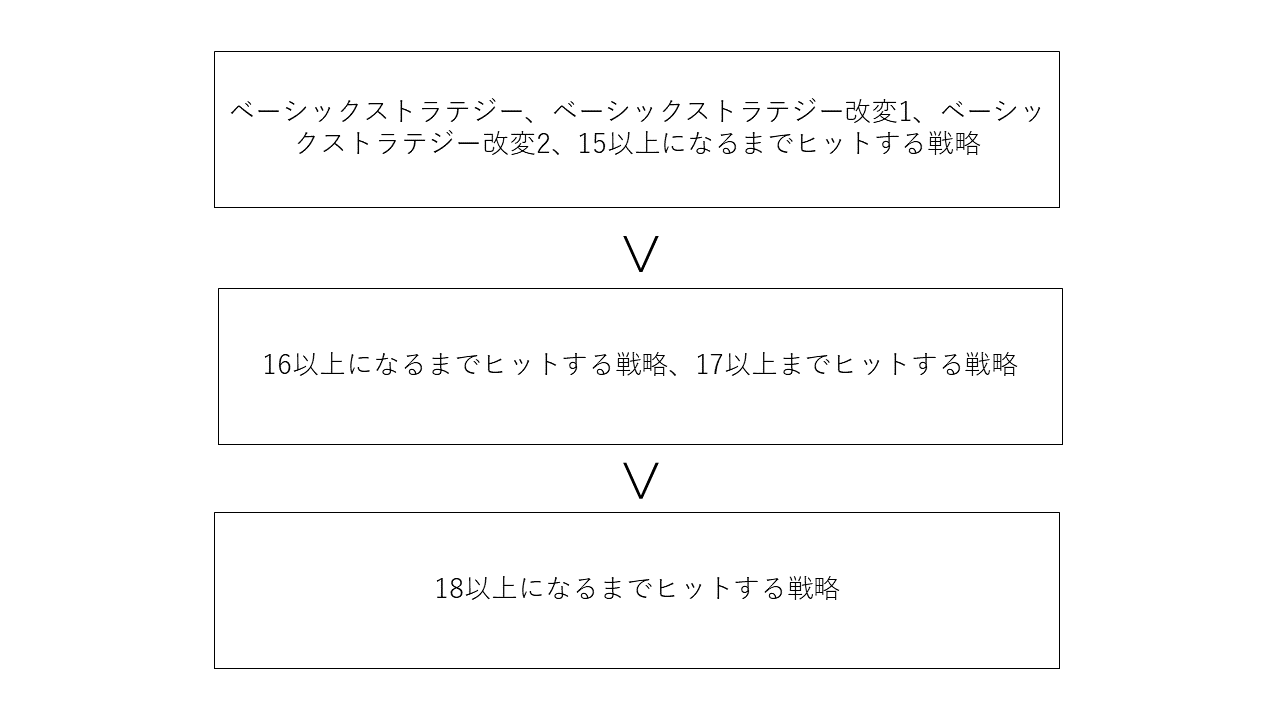
\includegraphics[width=0.7\linewidth]{./figure/statistics-rate1}
  \caption{デック数無限の勝率順\label{rate1}}
 \end{center}
\end{figure}

デック数1の場合、ベーシックストラテジー、ベーシックストラテジー改変1とベーシックストラテジー改変2の3つに勝率に有意な差が存在しない。15以上になるまでヒットする戦略、16以上になるまでヒットする戦略と18以上になるまでヒットする戦略の3つに有意な差が存在しない。これらを勝率の高い順に戦略を並べると、ベーシックストラテジーとベーシックストラテジー改変1ベーシックストラテジー改変2の戦略、15と16と18以上になるまでヒットする戦略、17以上になるまでヒットする戦略となる。これを図\ref{rate2}で示す。

\begin{figure}[H]
 \begin{center} 
  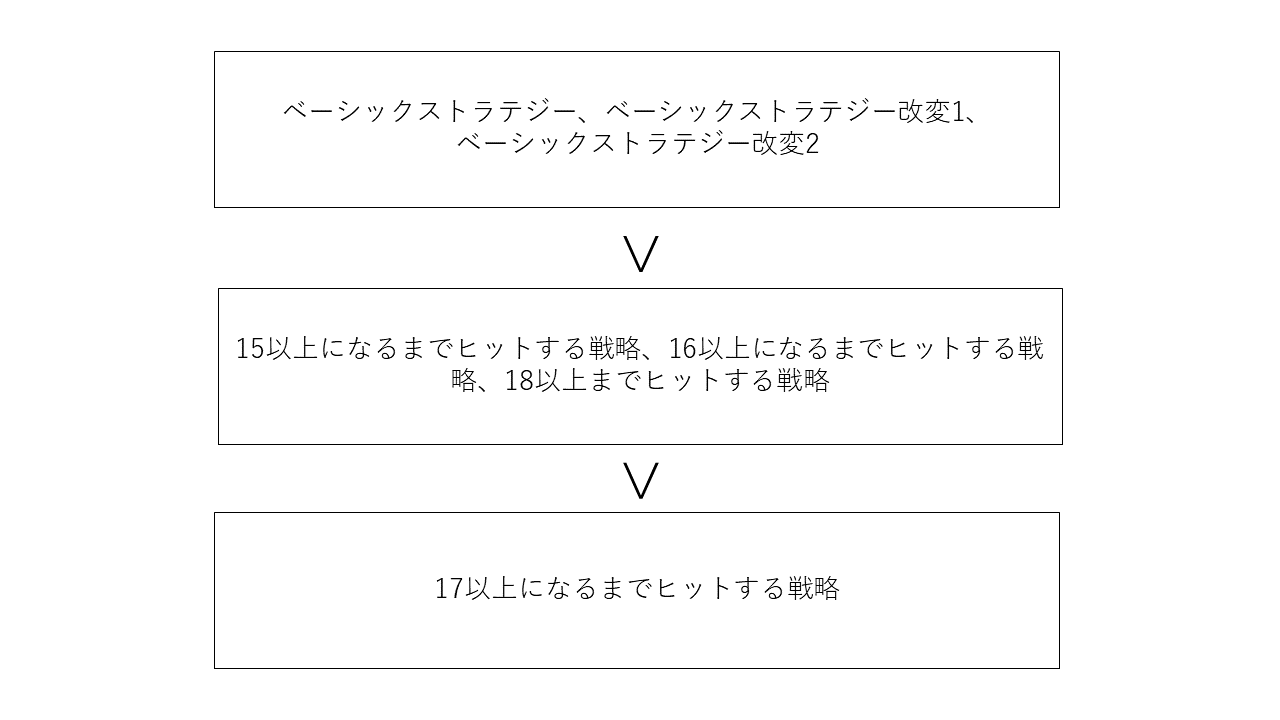
\includegraphics[width=0.7\linewidth]{./figure/statistics-rate2}
  \caption{デック数1の勝率順\label{rate2}}
 \end{center}
\end{figure}

\bunseki{柿崎大輝}
